\section{Menu flowchart and explanation~\ref{fig:menu}}
\begin{figure}
    \centering 
    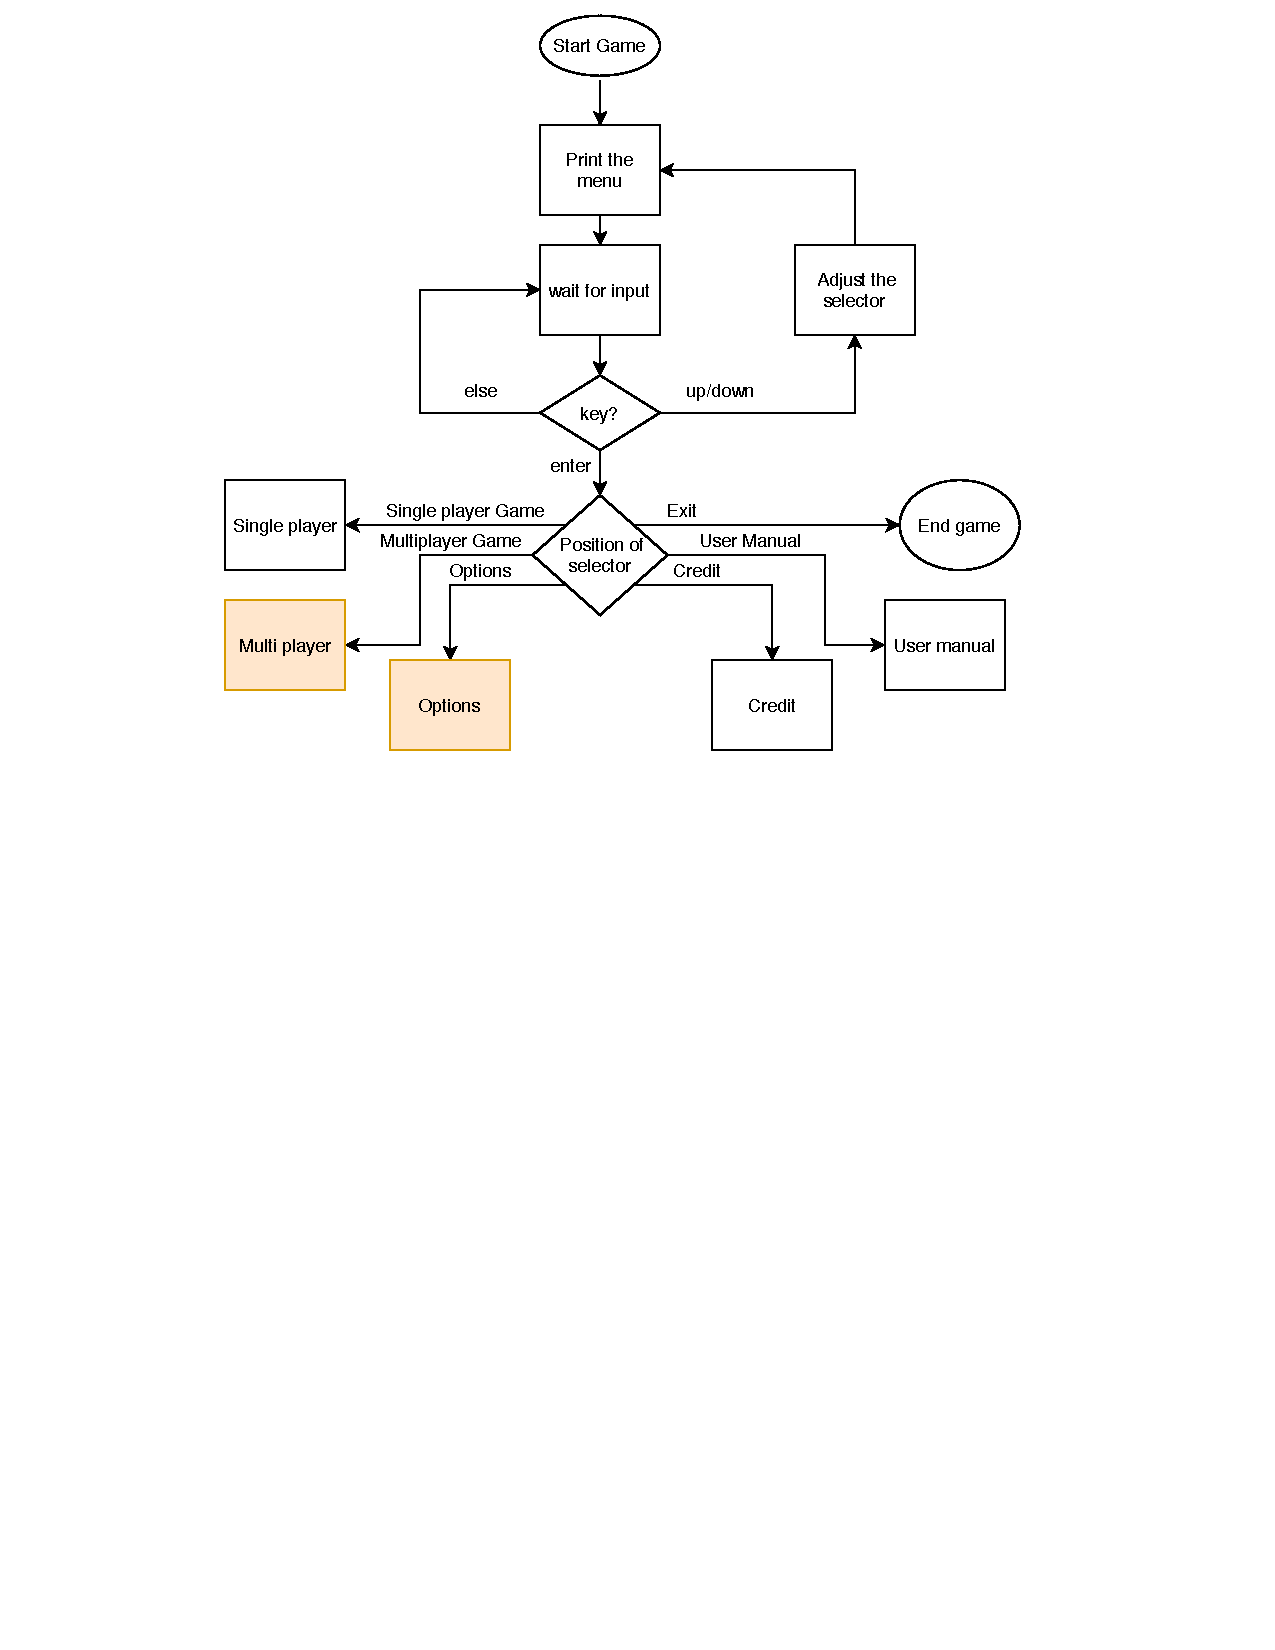
\includegraphics[width=0.8\columnwidth]{menu.pdf}
    \caption{Menu flowchart. white blocks are implemented in first release and \textcolor{orange}{orange} blocks are implemented in second release. }
    \label{fig:menu}
\end{figure}

This section explains the flow of our program since execution starts until it finishes. 
As it is shown in Figure \ref{fig:menu}, initially, we print a menu for the game. There are multiple choices on the game menu and user can go through each of them and press enter to select one. So, program is waiting for the user to press up/down/enter key. Showing the menu items is handle in a graphic library (SDL).
Next step decides what to do based on the user's choice. 
As we've seen in Figure~\ref{fig:menu}, we may go on six different scenarios: user manual, single player, multiplayer, options, credit and end game/exit which will be explained in detail in the coming sections.

\subsection{Menu functions prototype}
In this section we define the required functions prototypes and its relation to flow chart. Comments above each function mention the associated block, the release, and assignee.
\begin{minted}{c}
#define MAX_ITEM_SIZE 100              /**< maximum legth of menu item*/

/**
 * @enum menu_items_t
 * The enumeration of menu items.
 */
typedef enum menu_items {
	MENU_ITEM_USER_MANUAL,
	MENU_ITEM_SINGLE_PLAYER,
	MENU_ITEM_MULTI_PLAYER,
	MENU_ITEM_OPTIONS,
	MENU_ITEM_CREDIT,
	MENU_ITEM_EXIT,
	MENU_ITEM_NUM_OF_ITEMS
} menu_items_t;

/**
 * @typedef item_t
 * A structure represents items' name.
 */
typedef struct item {
	char str[MAX_ITEM_SIZE];    /**< the name of the item in the menu*/
} item_t;

/**
 * @typedef menu_t
 * A structure represents menu item.
 */
typedef struct menu {
	menu_items_t selector;
	item_t items[MENU_ITEM_NUM_OF_ITEMS ];
} menu_t;

/**
 * @brief The main function which handle the whole program.
 * @author Pari 
 * Wrote in release one and updated for release two.
 *
 * The main function initialize a SDL window, print menu items,
 * wait for up/ down/ enter/ backspace/ quit input keys from the user and
 * call associated functions accordingly.
 * @return 0 in success.
 */
int main()

/**
 * @brief Prints user manual on an input window.
 * @author wrote by Jin, updated by Pari.
 * Wrote in release one and updated for release two.
 * @param[in] p_window a SDL window which is passed from the main function.
 * @return bool if window is quit or back_space key is pressed, return true.
 */
bool user_manual(SDL_Window* p_window);

/**
 * @brief single_player function
 * @author Pari
 * First release.
 * This is the main function which handle single player mode.
 * Different functions are called here: first a map file is loaded and then
 * according to the input key different entities is updated and a view will be generated.
 * A timer is initialized to update every thing in each TIMER_INTERVAL seconds.
 * @param[in] p_window a SDL window which is passed from the main function.
 * @param[in] difficulty game difficulty specify the map file that should be loaded.
 * @return bool if window is quit or back_space key is pressed, return true.
 */
bool single_player(SDL_Window* p_window, option_items_t difficulty);

/**
 * @brief multi_player function
 * @author Jin 
 * Second release
 * This is the main function which handle multi player mode.
 * Different functions are called here: first a map file is loaded and then
 * according to the input key different entities is updated and a view will be generated.
 * A timer is initialized to update every thing in each TIMER_INTERVAL seconds.
 * @param[in] p_window a SDL window which is passed from the main function.
 * @param[in] difficulty game difficulty specify the map file that should be loaded.
 * @return bool if window is quit or back_space key is pressed, return true.
 */
bool multi_player(SDL_Window* p_window,option_items_t difficulty);

/**
* @brief Handles user input to choose between difficulty levels.
* @author Jaser
* Second release
* This function show you different level of difficulty and let
* user to choose between difficulty levels using return/enter key.
*
* @param[in] p_window A SDL window is passed to the function.
* @param[out] p_option_items final selected item.
* @return bool if window is quit or back_space key is pressed, return true.
*/
bool options(SDL_Window* p_window, option_items_t* p_option_items);

/**
 * @brief Prints Credits Information on the input window.
 * @author Mahsa
 * @param[in] p_window a SDL window which is passed from the main function.
 * @return bool if window is quit or back_space key is pressed, return true.
 */
bool credit(SDL_Window* p_window);

/**
* @brief Prints the game start up menu on an input SDL window.
* @author Pari
* First release.
* @param[in] p_window A SDL window is passed to the function.
* @param[in] p_menu A structure represents menu items.
* @return void
*/
void print_menu(SDL_Window* p_window, menu_t* p_menu);
\end{minted}